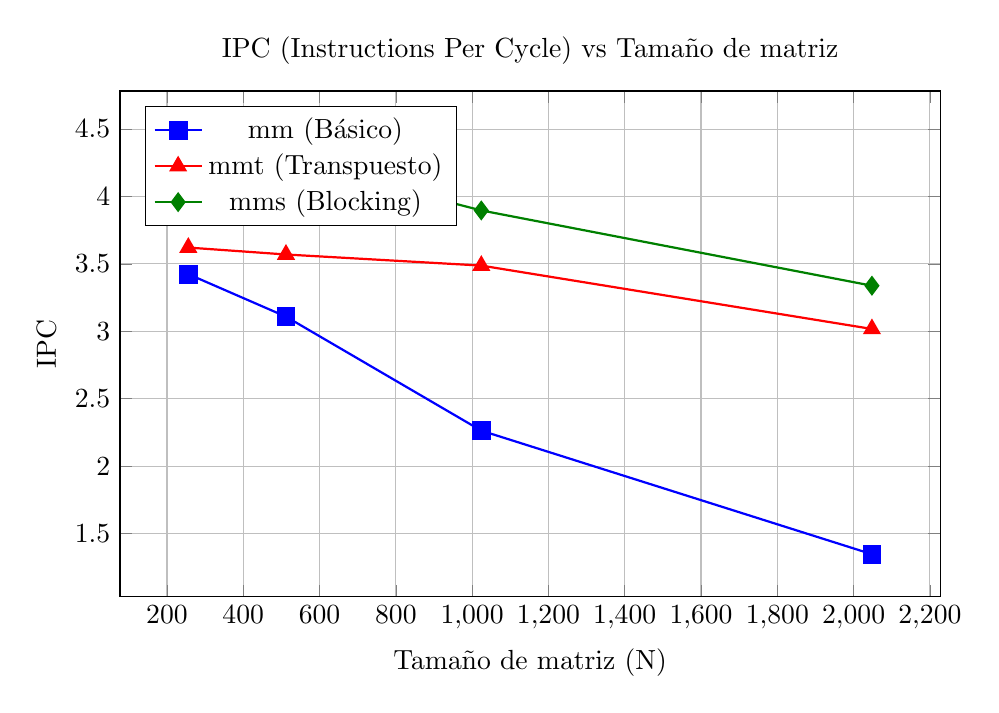
\begin{tikzpicture}
    \begin{axis}[
        title={IPC (Instructions Per Cycle) vs Tamaño de matriz},
        xlabel={Tamaño de matriz (N)},
        ylabel={IPC},
        legend pos=north west,
        grid=major,
        width=12cm,
        height=8cm,
    ]
        \addplot[
            color=blue,
            mark=square*,
            thick,
            mark size=3pt,
        ]
        coordinates {
            (256, 3.424114)
            (512, 3.109029)
            (1024, 2.263666)
            (2048, 1.347255)
        };
        \addlegendentry{mm (Básico)}
        \addplot[
            color=red,
            mark=triangle*,
            thick,
            mark size=3pt,
        ]
        coordinates {
            (256, 3.621219)
            (512, 3.569818)
            (1024, 3.487592)
            (2048, 3.017645)
        };
        \addlegendentry{mmt (Transpuesto)}
        \addplot[
            color=green!50!black,
            mark=diamond*,
            thick,
            mark size=3pt,
        ]
        coordinates {
            (256, 4.470291)
            (512, 4.270219)
            (1024, 3.896507)
            (2048, 3.338437)
        };
        \addlegendentry{mms (Blocking)}
    \end{axis}
\end{tikzpicture}
